%-*- program: xelatex -*-
%-*- program: biber -*-
%-*- program: xelatex -*-

\documentclass[
    sigplan,
    10pt,
    review, % Note: remove the [review] option for the final document.
    natbib=false % Note: This ishere to be able to use Biber.
 ]{acmart}
%\let\citename\relax

\settopmatter{printfolios=true,printccs=false,printacmref=false}

\acmConference[DLS'18]{Dynamic Languages Symposium}{November~6, 2018}{Boston, MA, USA}
\acmYear{2018}
\acmISBN{} % \acmISBN{978-x-xxxx-xxxx-x/YY/MM}
\acmDOI{} % \acmDOI{10.1145/nnnnnnn.nnnnnnn}
\startPage{1}

\setcopyright{none}

\bibliographystyle{ACM-Reference-Format}

\usepackage{booktabs}
\usepackage{subcaption}

\usepackage[
   backend=biber,
   bibencoding=utf8,
   style=numeric,
   hyperref=true,
   % citestyle=authoryear-comp,
   backref=false,
   sortlocale=en,
   url=true,
   doi=false,
   eprint=false
 ]{biblatex}
\addbibresource{biblio.bib}

\usepackage{minted}
\setminted{
    encoding=utf8,
    fontsize=\small,
    breaklines,
    linenos,
    numbersep=.6em,
    autogobble
  }

\usepackage{tikz}
\usetikzlibrary{positioning}

\tikzset{
	box/.style = {
		draw = black,
        fill = white,
		rectangle,
		rounded corners = 2pt,
		text centered,
		minimum height = 5mm,
		minimum width = 10mm
	}
}

\usepackage{todonotes}
\newcommand\mb[1]{\todo[color=purple!20,size=\scriptsize]{#1}}
\newcommand\mbi[1]{\todo[color=purple!20,inline]{#1}}
\newcommand\et[1]{\todo[color=blue!20,size=\scriptsize]{#1}}
\newcommand\eti[1]{\todo[color=blue!20,inline]{#1}}
\newcommand\td[1]{\todo[color=green!20,size=\scriptsize]{#1}}
\newcommand\tdi[1]{\todo[color=green!20,inline]{#1}}

\setlength{\marginparwidth}{15mm} % Note: This is only temporary, to have notes more readable. It should be removed before submitting.

\newcommand\ignore[1]{}

\newcommand\CoqR{CoqR}

\begin{document}

\title{A Trustworthy Mechanized Formalization of R}

\author{Martin Bodin}
\orcid{0000-0003-3588-3782}
\affiliation{
  %\position{}
  \department{Center for Mathematical Modeling \& \\
  Computer Science Department}
  \institution{University of Chile}
  % \streetaddress{Beauchef 851}
  % \city{Santiago}
  % \state{State1}
  % \postcode{Post-Code1}
  % \country{Chile}
}
\email{mbodin@dim.uchile.cl}

\author{Tom{\'a}s Diaz}
% \authornote{with author2 note}
% \orcid{nnnn-nnnn-nnnn-nnnn}
\affiliation{
  \position{Pleiad Lab}
  \department{Computer Science Department}
  \institution{University of Chile}
  % \streetaddress{Beauchef 851}
  % \city{Santiago}
  % \state{State2a}
  % \postcode{Post-Code2a}
  % \country{Chile}
}
\email{tdiaz@dcc.uchile.cl}

\author{{\'E}ric Tanter}
% \authornote{with author2 note}
% \orcid{nnnn-nnnn-nnnn-nnnn}
\affiliation{
  \position{Pleiad Lab \& IMFD Chile}
  \department{Computer Science Department}
  \institution{University of Chile}
  \streetaddress{Beauchef 851}
  % \city{Santiago}
  % \state{State2a}
  % \postcode{Post-Code2a}
  % \country{Chile}
  \thanks{{\'E.} Tanter is partially funded by the Millenium Institute for Foundational Research on Data (IMFD Chile)}
}
\email{etanter@dcc.uchile.cl}

\begin{abstract}
The R programming language is very popular for developing statistical software and data analysis, thanks to rich libraries, concise and expressive syntax, and support for interactive programming. Yet, the semantics of R is fairly complex, contains many subtle corner cases, and is not formally specified. This makes it difficult to fully trust R programs. In this work, we develop a big-step operational semantics for R in the form of an interpreter written in the Coq proof assistant. We ensure the trustworthiness of the formalization by introducing a monadic encoding that allows the Coq interpreter, \CoqR, to be in direct visual correspondence with the reference R interpreter, GNU~R. Additionally, we provide a testing framework that supports systematic comparison of \CoqR{} and GNU~R. In its current state, \CoqR{} covers the core of the R language as well as numerous additional features, making it pass a significant number of realistic test cases from the GNU~R and FastR projects. To exercise the formal specification, we prove in Coq the preservation of memory invariants in selected parts of the interpreter. This work is an important first step towards a robust environment for 
formal verification of R programs.
\end{abstract}

% % %% 2012 ACM Computing Classification System (CSS) concepts
% % %% Generate at 'http://dl.acm.org/ccs/ccs.cfm'.
% \begin{CCSXML}
%   <ccs2012>
%     <concept>
%       <concept_id>10003752.10010124.10010131.10010133</concept_id>
%       <concept_desc>Theory of computation~Denotational semantics</concept_desc>
%       <concept_significance>500</concept_significance>
%     </concept>
%     <concept>
%       <concept_id>10011007.10011006.10011066.10011070</concept_id>
%       <concept_desc>Software and its engineering~Application specific development environments</concept_desc>
%       <concept_significance>300</concept_significance>
%     </concept>
%     <concept>
%       <concept_id>10011007.10011074.10011099.10011692</concept_id>
%       <concept_desc>Software and its engineering~Formal software verification</concept_desc>
%       <concept_significance>100</concept_significance>
%     </concept>
%   </ccs2012>
% \end{CCSXML}

% \ccsdesc[500]{Theory of computation~Denotational semantics}
% \ccsdesc[300]{Software and its engineering~Application specific development environments}
% \ccsdesc[100]{Software and its engineering~Formal software verification}
% % %% End of generated code

% \keywords{R, Coq, Formalization, Testing}

\maketitle

\section{Introduction}
\label{sec:intro}

% R is used a lot.
The R programming language~\parencite{R, ihaka1996r, Rwebsite}
has gotten a lot of traction in recent years, being used by millions of users in areas as varied as biology and finance. This diversity among R programmers results in largely different programming styles. In fact, the language itself is community driven and reflects this diversity.
% R is complex and we need to certify R softwares.
The R programming language is meant to be both expressive and powerful,
able to express complex notions in few keystrokes.
This sometimes comes at the cost of readability and predictability. Indeed,
the semantics of R is subtle and contains numerous corner cases that can result in unexpected behavior.

The reasons for these corner cases are numerous, ranging from backward compatibility to the desire to accommodate the use of R as both a traditional programming language and an interactive shell.
Even a feature as basic as function calls can be the source of surprises in R.
Indeed, there are many ways to call a function, and in particular there are two ways to provide an argument: either by position or by name.\footnote{
    To simplify, we ignore the \mintinline{R}{...} construct
    as well as default arguments, which both have non-trivial interactions with the other constructs.} While this per se is fairly common, the way R supports it is not; in particular it supports matching names {\em by prefix}.
%
To illustrate some subtleties that follow from this feature,
Figure~\ref{fig:calls} defines a function \mintinline{R}{f} that concatenates its three arguments. The first call associates arguments by position, and the second by name. The third call mixes both mechanisms, and exploits the prefix feature: \mintinline{R}{d} is associated to \mintinline{R}{de}
because it is the only argument whose name starts with \mintinline{R}{d}.
Now, if more than one argument matches by prefix,
then R rejects the call and throws an error,
as in the fifth call in Figure~\ref{fig:calls}.
However, exact matches are not counted in this process:
in the fourth call,
the name \mintinline{R}{ab} is an exact match
and thus only the argument \mintinline{R}{abc}
is left to be associated to \mintinline{R}{a},
leading to no error thrown.

\begin{figure}[t]
\begin{minted}{R}
f <- function (abc, ab, de) { c (abc, ab, de) }
f(1, 2, 3)           # By position
f(de=3, abc=1, ab=2) # By name
f(1, d=3, 2)         # Mixed
f(3, a=1, ab=2)      # a is associated to abc
f(a=3, 1, 2)         # error: several prefixes
\end{minted}
\caption{Exploring function calls in R.}
\label{fig:calls}
\end{figure}

Such subtle behaviors are numerous in R~\parencite{RInferno}.
Debugging tools exist~\parencite{mcpherson2014},
but they cannot always compensate for the complex semantics of R.
Consequently, surprising bugs occur in R programs
and fully trusting such programs can be difficult.
%
% We need a formalization of the language.
Formal methods offer a solution to the trust issue:
proof assistants such as Coq~\parencite{Coq} enable us
to formally prove program properties with a high amount of trust.
But to formally prove that an R program meets its specification,
we first need a formal semantics of R. While there exists a language definition document~\parencite{R}, this document is unfit for serving as the basis of a verification effort; it is both a specification effort and a manual, written in plain English, with ambiguities and incomplete at times. Additionally, we found several mismatches between the text description and the behavior of the reference interpreter, GNU~R~\parencite{Rwebsite}.\footnote{For instance, according to the language definition, \mintinline{R}{if ("TRUE") 42} should raise an error, whilst the interpreter returns \mintinline{R}{42}.}
Crucially, the formal semantics should account for all the subtle cases of the R semantics, such as function call conventions described above, implicit type conversions, and so on.
This is necessary because these corner cases are indeed a typical place were bugs appear and are hard to track.
A complete semantics for the full R language will inevitably be complex,
because of the large amount of such corner cases.

% This formalization is quite large, and we need to certify it.
This complexity in turn raises a meta-trust issue:
how can a large semantics (and consequently the proofs made from it)
be trusted? Being able to relate a formalism to {\em trust sources} is a crucial aspect of the formalization process, and often requires a large amount of work to be done properly~\parencite{leroy2014pip}. This challenge has been faced repeatedly in attempts to provide formal foundations to JavaScript, for instance.
%
Some formalization approaches like $\lambda_{JS}$~\cite{Guha2010} and KJS~\cite{kjs} augment trust through extensive testing and comparison with existing implementations. JSCert~\parencite{popl14jscert} only uses testing, without directly comparing to an existing implementation, but further augments trust through the notion of a so-called {\em eyeball correspondence}, i.e.~a line-to-line syntactic connection, between the formalization (in Coq) and the ECMAScript specification (in English and pseudo-code).

\paragraph{Contributions.}
We present \CoqR{}, a trustworthy formalization of the R programming language in the Coq proof assistant.
The formalization is a big-step operational semantics, in the form of an interpreter (Section~\ref{sec:coq:interp}).
%
We say that this interpreter is {\em trustworthy} because we have followed two complementary techniques to maximize trust: eyeball correspondence, and testing.

First, the Coq interpreter has been written using a monadic encoding that allows for a direct eyeball correspondence with the C source code of GNU~R~\parencite{Rwebsite}. In the absence of a standardized formal semantics, GNU~R is the reference point that defines what R really is. Note that other alternative implementations of R, such as FastR~\parencite{kalibera2014fast}, also treat GNU~R as the ground truth.

Second, we have developed a testing framework that streamlines the process of running both the Coq interpreter and GNU~R on a set of test cases and report on mismatches and errors, among others (Section~\ref{sec:testing:architecture}). We use several test suites to measure the advancement of the \CoqR{} implementation. 
% the test suite of GNU~R itself ($\sim$3,600 loc), a test suite of the FastR implementation ($\sim$1,300 loc)~\parencite{kalibera2014fast}, and a test suite that we developed to exercise corner cases ($\sim$1,100 loc).

Additionally, we report on the process of scaling up our interpreter in order to be able to load existing R libraries (Section~\ref{sec:library}), in particular the R base library. Finally, we report on a proof effort to establish that memory invariants are preserved during execution, including some specific proof automation (Section~\ref{sec:proofs}).
%
Section~\ref{sec:related:work} discusses related work and Section~\ref{sec:conclusion} concludes.

The current implementation of \CoqR{} is not feature complete; R is a very large programming language and achieving 100\% coverage of the language and its main libraries is a huge implementation effort, which would need involvement from the R community at large. The contribution of this work is to provide realistic foundations of a trustworthy R formalization in Coq. First, the interpreter covers the core of the language and over 100 additional features. It is implemented in an extensible manner, following the architecture of GNU~R itself. Second, the testing infrastructure we provide is designed to help drive the development effort towards the most pressing missing features. At present, the \CoqR{} implementation passes approximately half \et{update - and what about our own test suite? 100\%?} of the GNU~R and FastR test suites, which is realistic enough to support the claim that, given more engineering power, our approach can scale up to the full language and its main libraries.



% Given the size of our formalization,
% we consider this part to be the most important of our contributions.

% The development presented here, including the Coq interpreter, the testing framework, and the tests, is available online at:\\
% \url{https://github.com/Mbodin/proveR/releases/tag/DLS2018}\todo{make this tag exist on Github}.

% % Contributions.
% We introduce \CoqR{}

% a formalization of the R programming language in the Coq proof assistant.
% This is a continuation of a previous work~\parencite{CoqRCoqPL},
% \mb{Political choice here: is it a good idea to cite this previous work?}\et{no, skip - this wasn't a technical result, just a progress report/position paper}
% in which we formalised a small core of the R language.
% The additional contribution of this paper is the additional
% of a non-trivial quantity of R features,
% which enabled us to import R libraries.
%
%
% This two-factors method is very close to the one of JSCert,
% which we discuss in Section~\ref{sec:related:work}.



% % Outlines.
% \eti{update when paper is stable:}
% This paper is organized as follows.
% Section~\ref{sec:coq:interp} presents the Coq interpreter.
% In particular, Section~\ref{sec:eyeball:closeness} presents
% how this semantics is syntactically close to the C source code of R.
% Section~\ref{sec:testing:architecture} then presents our testing architecture.
% Not only this architecture is used as a way to relate our semantics
% with R reference interpreter,
% it also provided immediate benefits during the development of the semantics.
% Section~\ref{sec:driving:development} presents these benefits.
% The testing results are shown in Section~\ref{sec:test:results}.
% Finally, Section~\ref{sec:proofs} presents some proofs that have been done
% using our language formalization.

\section{\CoqR: An R Interpreter in Coq}
\label{sec:coq:interp}

We develop the formal semantics of R in the form of an interpreter defined in Coq; therefore, this is a big-step operational semantics.
Operational semantics written as a Coq recursive function is usually not the best fit for Coq proofs---an inductive definition of the operational semantics is usually more convenient for reasoning---but our approach comes with a crucial advantage: it can be run, and thus tested.
%
In this section, we show how we define the Coq interpreter in order to achieve the first of the two mechanisms in place for trust, namely the eyeball correspondence with the GNU~R interpreter.

\subsection{Bridging the Gap between C and Coq}
\label{sec:monad}

The basic principle of the eyeball correspondence is that every one or two lines of the Coq interpreter should correspond to one or two lines of the C reference interpreter.

Of course, achieving a close correspondence between C and Coq versions of the same program is quite challenging, because C and Coq are widely different programming languages:
Coq is purely functional
whilst global side-effects are frequent in C.
Furthermore, Coq is designed to reject any function
whose behavior is not entirely defined
(it is for instance impossible to miss a case in a pattern-matching),
whilst C is known for its undefined behaviors.
Finally, contrary to C, Coq programs are required to terminate.

\begin{figure}[t]
\begin{minted}{Coq}
Inductive result (A : Type) :=
  | result_success : state -> A -> result A
  | result_error : state -> string -> result A
  | result_longjump : state -> context -> result A
  | result_impossible : state -> string -> result A
  | result_not_implemented : string -> result A
  | result_bottom : state -> result A.
\end{minted}
\caption{The result monad.}
\label{fig:result}
\end{figure}

In order to limit the impact that these differences can have on the eyeball correspondence, we introduce a {\em result monad}, which combines both the state, error, and fuel monads (Figure~\ref{fig:result}), and allows us to program in Coq ``as if it were C''.%
%
\footnote{Recall that monads allow purely functional programs to account for effectful computation, by means of implicit threading of information using a {\em binder}~\parencite{wadler:mscs1992}. For instance, the state monad threads a piece of state through a functional computation, accessible via monadic operations like \mintinline{Coq}{put} and \mintinline{Coq}{get}, thereby simulating a mutable store.}
More precisely, the result monad features the following constructors:\footnote{The result monad is similar to the one used in the JSExplain project~\parencite{JSExplain}, which aims at defining a JavaScript interpreter in Coq, readable by non-specialists.
}
\begin{itemize}
\item The main constructor is \mintinline{Coq}{result_success}, used when a computation is successful.
In addition to the result (of type \mintinline{Coq}{A} in the definition),
it carries the global state (of type \mintinline{Coq}{state}). (We describe the representation of state later on in this section.)
%
\item The constructor \mintinline{Coq}{result_error} is meant to catch
errors thrown by GNU~R, for instance an R runtime typing error:
these errors are not catchable and immediately end the execution.
A \mintinline{Coq}{string} is provided to help the debugging process.
%
\item The constructor \mintinline{Coq}{result_longjump}
corresponds to a call to the \mintinline{C}{longjmp}
C function in GNU~R source code.
It only appears in constructs involving non-local jumps,
such as \mintinline{R}{break} or \mintinline{R}{return}.
% The \mintinline{C}{longjmp} jumps to the corresponding
% \mintinline{C}{setjmp} function,
% which typically appears in loops and function calls.
% For instance, Figure~\ref{fig:do_repeat:c} shows the C code
% of the \mintinline{R}{repeat} feature of R,
% which keeps on executing its argument.
% Once a \mintinline{C}{longjmp} is executed
% (for instance by a \mintinline{R}{break}),
% the current program point is set to be Line~\ref{line:do_repeat:c:setjmp}.
% The \mintinline{C}{setjmp} function then returns
% the argument of the \mintinline{C}{longjmp}.
% % This enables the interpreter to differenciate on the kind of non-local behavior.
% We needed to add a special constructor
% to translate this specific behavior of C.
%
\item Unspecified C behaviors
(such as dereferencing an invalid pointer)
are translated into
\mintinline{Coq}{result_impossible}.
Getting this result immediately ends the Coq interpreter:
it is meant to be unreachable.
Observing such a result would mean that a bug in GNU~R has been found, which could possibly be undetectable by running GNU~R due to a C compiler optimization.\footnote{At this date, we have not encountered this situation (yet?).}
% \et{has this happened? I guess not}
% \mbi{No it hasn't. What I meant is that in \CoqR{}, undefined behaviors always result in a special error,
%      whilst in GNU~R, this could result in a silent error due to compiler optimizations:
%      we are in theory able to catch ``bugs'' that direct testing on GNU~R wouldn't be able to catch.}
%
\item Given the size and complexity of the R language, it is important to be able to execute the Coq interpreter without it being fully complete.
The specific constructor \mintinline{Coq}{result_not_implemented} is thus important
for development; it is treated specifically in our testing framework, for instance to help identity which features one should focus on next.
%
\item Finally, \mintinline{Coq}{result_bottom} is returned
to end the execution when reaching the maximum number of executed instructions
(also called \emph{fuel}). This is meant to artificially make our interpreter terminate, despite the fact that the interpreted R program may not.
\end{itemize}

% \begin{figure}
% \begin{minted}[escapeinside=@@]{C}
% SEXP do_repeat (EXP* call, EXP* op,
%                 EXP* args, EXP* rho){
%   EXP* body;
%   RCNTXT cntxt;
%   checkArity (op, args);
%   body = CAR (args);
%   begincontext (&cntxt, CTXT_LOOP, rho, R_BaseEnv);
%   if (setjmp (cntxt.cjmpbuf) != CTXT_BREAK) {@\label{line:do_repeat:c:setjmp}@
%     for (;;) eval (body, rho);
%   }
%   endcontext (&cntxt);
%   return R_NilValue;
% }
% \end{minted}
%     \caption{C code of the \mintinline{C}{do_repeat} function}
%     \label{fig:do_repeat:c}
% \end{figure}

The result monad is associated with a monadic binder,
written \mintinline{Coq}{let%success}.
This binder expects its argument to evaluate to a result of the form
\mintinline{Coq}{result_success}. If so, it binds the carried result to a name, and transparently propagates the possibly-updated state.
All other kinds of results are transparently propagated to the top-level.
A similar monadic binder has been defined to handle
the special semantics of \mintinline{C}{setjmp}.
This obliviousness to global state, errors and non-termination is what enables a close correspondence between a program written in both languages.

% We believe that this helps to find bugs in \CoqR{}
% and to convey trust to the overall R semantics.

\begin{figure*}[t]
    \centering{}
\begin{subfigure}{.54\textwidth}
\begin{minted}{C}
EXP* do_attr (EXP* call, EXP* op,
              EXP* args, EXP* env){
  EXP* argList, car, ans;
  /* ... */
  int nargs = R_length (args);
  argList = matchArgs (do_attr_formals, args, call);
  PROTECT (argList);
  if (nargs < 2 || nargs > 3)
    error ("Wrong argument count.");
  car = CAR (argList);
  /* ... */
  return ans;
}
\end{minted}
    \caption{original C function}
    \label{fig:c:do_attr}
\end{subfigure}
\begin{subfigure}{.45\textwidth}
\begin{minted}{Coq}
Definition do_attr globals runs S
    (call op args env : EXP_pointer) :=
  let%success nargs :=
    R_length globals runs S args using S in
  let%success argList :=
    matchArgs globals runs S
      do_attr_formals args call using S in
  if nargs <? 2 || nargs >? 3 then
    result_error S "Wrong argument count."
  else
    read%list car, _, _ := argList using S in
    (* ... *)
    result_success S ans.
\end{minted}
    \caption{Coq translation}
    \label{fig:coq:do_attr}
\end{subfigure}
    \caption{Original C function and Coq translation of \mintinline{C}{do_attr}}
    \label{fig:do_attr}
\end{figure*}

\subsection{Eyeball Correspondence}
\label{sec:eyeball:closeness}


% % Definition of the line-to-line correspondence.
% One key specificity of this interpreter is that it has been designed
% to be similar to the original C source code of GNU~R.
% More precisely, they are related by a line-to-line correspondence
% (also called \emph{eyeball closeness})\et{is closeness a standard term here? (eyeball correspondence sounds better to me)}:
% every one or two lines of our interpreter
% correspond to one or two lines of the reference interpreter.
% %

By developing \CoqR{} as a monadic interpreter using the result monad introduced above, we are able to achieve an eyeball correspondence between the C and Coq interpreters. This correspondence is extremely helpful during development:
whenever a bug is encountered while testing, we localize the function responsible for the bug and then can directly and visually compare both interpreters. Such checks are quick and easy to perform, often leading to a quick fix of \CoqR{}.
%

Figure~\ref{fig:do_attr} shows an example of the eyeball correspondence that can be achieved using the result monad. Figure~\ref{fig:c:do_attr} shows a C function, and Figure~\ref{fig:coq:do_attr} its Coq translation.
The binder \mintinline{Coq}{let%success} is used when calling a function.
Thanks to the monadic encoding, the calls to \mintinline{Coq}{R_length}
and \mintinline{Coq}{matchArgs} may return an unsuccessful result, but the code does not need to be explicit about that possibility; the code after a call is only executed if the result denotes success. Similarly, the \mintinline{C}{return} statement from C is translated to \mintinline{Coq}{result_success}, and raising an error is performed using \mintinline{Coq}{result_error}.

The other differences that can be observed are several arguments systematically passed to each function (\mintinline{Coq}{globals}, \mintinline{Coq}{runs}, and \mintinline{Coq}{S}), as well as the use of
\mintinline{Coq}{read%list}
instead of \mintinline{C}{CAR} in the C version, and the fact that the use of the \mintinline{C}{PROTECT} macro is missing from the Coq version. We clarify each of these points in the following subsections.

% The \mintinline{Coq}{S} argument and the use
% are related to the modeling of the heap, discussed in Section~\ref{sec:coq:structure}.

% The \mintinline{Coq}{globals} argument is discussed in Section~\ref{sec:coq:structure}.

% The \mintinline{Coq}{runs} argument is related to dealing with non-termination, and is discussed in Section~\ref{sec:fuel}.



\begin{figure}
    \centering{}
    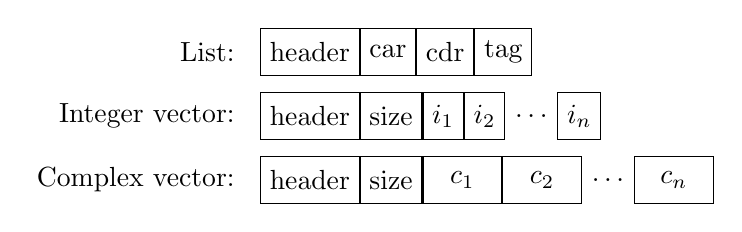
\begin{tikzpicture}
        \node [draw = black, rectangle, minimum height = 6mm, anchor = base] (hlist) {header} ;
        \node [draw = black, rectangle, minimum height = 6mm, anchor = base, right = 0pt of hlist] (car) {car} ;
        \node [draw = black, rectangle, minimum height = 6mm, anchor = base, right = 0pt of car] (cdr) {cdr} ;
        \node [draw = black, rectangle, minimum height = 6mm, anchor = base, right = 0pt of cdr] (tag) {tag} ;
        \node [left = 2mm of hlist] (nlist) {List:} ;

        \node [draw = black, rectangle, minimum height = 6mm, anchor = base, below = 2mm of hlist] (hvector1) {header} ;
        \node [draw = black, rectangle, minimum height = 6mm, anchor = base, right = 0pt of hvector1] (size1) {size} ;
        \node [draw = black, rectangle, minimum height = 6mm, anchor = base, right = 0pt of size1] (i1) {\(i_1\)} ;
        \node [draw = black, rectangle, minimum height = 6mm, anchor = base, right = 0pt of i1] (i2) {\(i_2\)} ;
        \node [anchor = base, right = 0pt of i2] (i3) {\(\ldots\)} ;
        \node [draw = black, rectangle, minimum height = 6mm, anchor = base, right = 0pt of i3] (in) {\(i_n\)} ;
        \node [left = 2mm of hvector1] (nvector1) {Integer vector:} ;

        \node [draw = black, rectangle, minimum height = 6mm, anchor = base, below = 2mm of hvector1] (hvector2) {header} ;
        \node [draw = black, rectangle, minimum height = 6mm, anchor = base, right = 0pt of hvector2] (size2) {size} ;
        \node [draw = black, rectangle, minimum height = 6mm, minimum width = 1cm, anchor = base, right = 0pt of size2] (c1) {\(c_1\)} ;
        \node [draw = black, rectangle, minimum height = 6mm, minimum width = 1cm, anchor = base, right = 0pt of c1] (c2) {\(c_2\)} ;
        \node [anchor = base, right = 0pt of c2] (c3) {\(\ldots\)} ;
        \node [draw = black, rectangle, minimum height = 6mm, minimum width = 1cm, anchor = base, right = 0pt of c3] (cn) {\(c_n\)} ;
        \node [left = 2mm of hvector2] (nvector2) {Complex vector:} ;
    \end{tikzpicture}
    \caption{Basic language elements in memory}
    \label{fig:basic:language:elements}
\end{figure}

\subsection{Modeling the Heap}
\label{sec:heap}

% Basic language elements.
We now describe how we modeled GNU~R's heap.
Although the underlying language is C,
GNU~R has been designed with a specific structure in mind~\parencite{R}.
Almost all objects manipulated by the interpreter
are called \emph{basic language elements},
or \mintinline{C}{EXP} in C.
Each of them are composed of a header and some data.
%
The header stores the type of the basic language element,
a list of attributes,
as well as several mostly-boolean informations
(for instance whether it can be safely updated in place).
There are \(24\) different types of basic language elements in R,
\(9\) of which being different kinds of vectors.
%
The stored data depends on the type of the element.
For instance, lists contain three pointers:
one to the first element (named \mintinline{Coq}{car}),
to the queue of the list (\mintinline{Coq}{cdr}),
and to an optional name for the first element (\mintinline{Coq}{tag}).
Vectors store their length,
followed by a C array in memory.
The size of this array depends both of its length
and the type of vector.
Figure~\ref{fig:basic:language:elements} illustrates this
with integer and complex vectors
(complexes are composed of two floats).
%
The way memory is used in C
makes it easy to unguardedly access a cell out of bounds,
which would lead to an undefined behavior.



% Guarded accesses in Coq to represent unguarded accesses in C.
This is an issue,
as we cannot directly translate unguarded C accesses into Coq:
we need a model of the heap.
Figure~\ref{fig:EXP} shows how we defined \mintinline{Coq}{EXP} in Coq.
Basic language elements are records storing a header
and data,
which in turn is defined as a sum type.
For instance, lists are defined by three pointers.
Vectors are records storing their length and a list:
in Coq, the data of vector is stored directly in the \mintinline{Coq}{EXP} structure
and not following it in memory as in C.

\begin{figure}
\begin{minted}{Coq}
Record ListStruct := make_ListStruct {
    list_carval : EXP_pointer ;
    list_cdrval : EXP_pointer ;
    list_tagval : EXP_pointer
  }.

Record Vector_EXP (A : Type) := make_Vector_EXP {
    Vector_length : nat ;
    Vector_data :> list A
  }.

Inductive EXPData :=
  | listExp : ListStruct -> EXPData
  | envExp : EnvStruct -> EXPData
  | EXP_VectorInteger : Vector_EXP int -> EXPData
  | EXP_VectorComplex : Vector_EXP complex -> EXPData
  (* ... *).
Coercion listExp : ListStruct >-> EXPData.
Coercion envExp : EnvStruct >-> EXPData.
(* ... *)

Record EXP := make_EXP {
    EXP_header :> EXPHeader ;
    EXP_data :> EXPdata
  }.
\end{minted}
    \caption{Basic language elements (\mintinline{C}{EXP}) in Coq}
    \label{fig:EXP}
\end{figure}

% About the use of coercions.
To ease readability, coercions have been used extensively.
Coercion is a mechanism to mark some constructors as implicit.
For instance, if Coq expects a \mintinline{Coq}{EXPData}
and is given a \mintinline{Coq}{ListStruct},
then the constructor \mintinline{Coq}{listExp} will be implicitly called
thanks to the corresponding line in Figure~\ref{fig:EXP}.
In the context of \CoqR{},
this is more than a simple syntactic notation
as it helps the eyeball correspondence
by hiding what is not present in C:
if one points to either a list or an environment,
the C notation to access its list or its environment is the same.
%
Of course, this implicit notation is only one-way:
given a \mintinline{Coq}{ListStruct},
we can convert it into an \mintinline{Coq}{EXPData},
but to perform the converse, we have to pattern-match
on the shape of the \mintinline{Coq}{EXPData}.
%
This pattern-matching is performed by specific monadic binders.
For instance in Figure~\ref{fig:coq:do_attr}, \mintinline{Coq}{read%list}
gets the \mintinline{Coq}{EXP} stored in the state \mintinline{Coq}{S}
and pointed by \mintinline{Coq}{argList},
then pattern-matches it as a list,
extracting the \mintinline{Coq}{car}, \mintinline{Coq}{cdr},
and \mintinline{Coq}{tag} fields.
If the pointer is not in the domain of the state \mintinline{Coq}{S}
or if the associated \mintinline{Coq}{EXP} object is not a list,
then \mintinline{Coq}{result_impossible} is returned:
this corresponds to an undefined behavior in C
(dereferencing an invalid pointer or accessing the wrong projection of a \mintinline{C}{union}).
The accesses in Coq are thus guarded by monadic binders,
whilst closely mimicking the unguarded accesses of C.


% Not modeling this part enabled us to focus on the computational part.
%
%
% At this stage, the reader should be able
% to compare the C and Coq programs of Figure~\ref{fig:do_attr}
% line by line.
% The rest of \CoqR{} was similarly defined.

\subsection{Dealing with Global Variables}
\label{sec:globals}

% Initialization of R and global variables.
The GNU~R interpreter features over \(80\) global variables that need initialization, and are subsequently unchanged.
The initialization of these internal variables
actually represents a large portion of the source code.
Even before importing any libraries, a lot of basic language elements
are created and stored in global variables.

For instance, the often-used variable \mintinline{C}{R_NilValue}
is set to be a list whose \mintinline{C}{car}, \mintinline{C}{cdr},
and \mintinline{C}{tag} fields point to \mintinline{C}{R_NilValue} itself.
This element is used instead of the \mintinline{C}{NULL} pointer
to mark any non-present element. Another important global variable is
\mintinline{C}{R_FunTab}, which is the {\em symbol table} that maps operation and function names to C functions implementing them. (We exploit this structuring of the interpreter for building \CoqR{} in an incremental manner---see Section~\ref{sec:coq:structure}.)

%
The initialization of global variable is fairly subtle. Most initializations perform local computations, calling core functions.
To avoid this circular dependency---which Coq would not accept---one could parametrize each core function by the value of the global variables it uses.
This would however not scale, considering the size of the project and the number of global variables involved.
%
Instead, we parameterize each function of \CoqR{} by a single \mintinline{Coq}{globals} environment, which is a mapping from a definite set of global variables to \mintinline{Coq}{EXP_pointer}. This additional argument can be seen in the Coq code of Figure~\ref{fig:coq:do_attr}: it is passed along at each call site.

To make definitions more convenient, we use coercions to make Coq implicitly perform a lookup in the \mintinline{Coq}{globals} environment whenever a global variable is read. Therefore, accessing global variables is transparent, as illustrated by the use of \mintinline{C}{do_attr_formals} in Figure~\ref{fig:coq:do_attr}.


\begin{figure*}
    \centering{}
\begin{subfigure}{.5\textwidth}
\begin{minted}{C}
  static EXP* do_attr_formals = NULL;
  if (do_attr_formals == NULL)
    do_attr_formals =
      allocFormalsList2 (install ("x"),
                         install ("which"));
\end{minted}
    \caption{C snippet}
    \label{fig:c:do_attr:formals}
\end{subfigure}
\begin{subfigure}{.49\textwidth}
\begin{minted}{Coq}
Definition do_attr_init globals runs S :=
  let%success x :=
    install globals runs S "x" using S in
  let%success which :=
    install globals runs S "which" using S in
  allocFormalsList2 globals S x which.
\end{minted}
    \caption{Coq translation}
    \label{fig:coq:do_attr:formals}
\end{subfigure}
    \caption{Another snippet of \mintinline{C}{do_attr} and its Coq translation}
    \label{fig:do_attr:formals}
\end{figure*}

% Static global variables.
\paragraph{Hidden global variables.} In fact \mintinline{C}{do_attr_formals} is a {\em hidden} global variable, introduced locally with the C \mintinline{C}{static} keyword inside the \mintinline{C}{do_attr} function. Such a variable is persistent across calls, just like a standard global variable.

In place of the first commented-out part in Figure~\ref{fig:c:do_attr}, the code actually defines the \mintinline{C}{static} variable \mintinline{C}{do_attr_formals}, as shown in Figure~\ref{fig:c:do_attr:formals}. Upon the first call of \mintinline{C}{do_attr}, the variable \mintinline{C}{do_attr_formals} is initialized by a basic language element. The value is kept across calls in order to avoid a costly reallocate at each call.
%
Observe that this pattern exactly follows the scheme of the other global variables: the variable is initialized once, and then never changes. Consequently, we treat such a \mintinline{C}{static} variable just like a global variable. We extracted out the part of \mintinline{C}{do_attr} that performs initialization, shown in Figure~\ref{fig:coq:do_attr:formals}.
This code is executed after the standard global variables are initialized.
% \et{what if the initialization of a static var uses some argument of the first call? does it ever happen?}\mb{I've never seen it. In such a case, I just add these variables in the state (this already happenned, but is rare).}


\subsection{Dealing with Non-Termination}
\label{sec:fuel}
% Structuring the fuel.
Another additional argument present in Figure~\ref{fig:coq:do_attr}
is the \mintinline{Coq}{runs} argument.
This argument aims at factorizing the fuel given to Coq functions
to make them artificially terminate.
The usual way to do this is to make each function check whether its fuel
reached \(0\), and if so return \mintinline{Coq}{result_bottom}.
It is however cumbersome to do that manually, and affects the eyeball correspondence, since such a check does not exist in C.
%
We solve this issue by following the same method as in JSCert:
instead of a fuel argument, each function takes a record \mintinline{Coq}{runs}.
This record stores all recursive functions as its projections.
Each recursive call in C is then translated by calling
the corresponding projection of the record,
as in a regular fix-point combinator.

For instance, Figure~\ref{fig:while_loop} shows the definition
of while loops in \CoqR{}.
First the \mintinline{Coq}{Runs} record is defined
with all the potentially looping functions.
A \mintinline{C}{while}-loop is obviously part of these functions.
We then define \mintinline{Coq}{while_loop} with an additional
argument \mintinline{Coq}{runs} of type \mintinline{Coq}{Runs}.
Line~\ref{line:runs_while:recursive:call} is the ``recursive'' call,
but instead of a recursive call,
we call the \mintinline{Coq}{while_loop} function stored
in the \mintinline{Coq}{runs} record.

\begin{figure}
\begin{minted}[escapeinside=@@]{Coq}
Record Runs : Type := Runs_intro {
    runs_while_loop : forall A, state -> A ->
      (state -> A -> result bool) ->
      (state -> A -> result A) -> result A ;
    runs_eval : state -> SEXP -> SEXP -> result SEXP ;
    (* ... *)
  }.

Definition while_loop runs A S (a : A) expr stat :=
  if%success expr S a using S then
    let%success a := stat S a using S in
    runs_while_loop runs S a expr stat@\label{line:runs_while:recursive:call}@
  else result_success S a.
\end{minted}
    \caption{Definition of loops as a fix-point combinator}
    \label{fig:while_loop}
\end{figure}

Once all functions have been defined,
we can define an inhabitant of \mintinline{Coq}{Runs}
by linking these functions to themselves.
In practice, we define \mintinline{Coq}{runs} using some fuel:
at each step, its projections are functions taking a \mintinline{Coq}{runs}
with less fuel as argument;
when reaching \(0\), all its projections systematically return \mintinline{Coq}{result_bottom}.
Figure~\ref{fig:runs} shows its Coq definition.
%
% \mb{Maybe we just don't want to speak about this:}
% \mbi{
% Note that the symbol table has to be one of the projections of \mintinline{Coq}{runs},
% otherwise a strangely-written function could in theory fetches itself from the symbol table
% and executes it, leading to an unwanted loop.
% Addition: this is called the “Landin’s knot”, but we probably still don’t want to speak about it ☺
% }
% %
In addition to passing the extra-argument argument, this idiom only requires one pattern-matching on fuel in the whole \CoqR{} interpreter; it is thus a very lightweight way to introduce termination.

\begin{figure}
\begin{minted}{Coq}
Fixpoint runs max_step globals : Runs :=
  match max_step with
  | O => {|
      runs_while_loop := fun _ S _ _ _ =>
        result_bottom S ;
      runs_eval := fun S _ _ =>
        result_bottom S ;
      (* ... *) |}
  | S n => {|
      runs_while_loop := fun A S (a : A) expr stat =>
        while_loop globals (runs n) A S a expr stat ;
      runs_eval := fun S e rho =>
        eval globals (runs n) S e rho ;
      (* ... *) |}
  end.
\end{minted}
    \caption{Definition of \mintinline{Coq}{runs} in Coq}
    \label{fig:runs}
\end{figure}


\subsection{Limitations}
% About garbage collection.
The use of the \mintinline{C}{PROTECT} macro in Figure~\ref{fig:c:do_attr} is missing in the Coq translation. This macro use performs a garbage collecting action, namely it saves the object \mintinline{C}{argList} from garbage collection.
At this stage, we chose not to model the garbage collection aspect of GNU~R in \CoqR{}. Indeed, garbage collection adds complexity to the interpreter, but is not supposed to affect the result of any computation. For now, we focus on the computational part of GNU~R.

% Ignored aspects.
% As stated in Section~\ref{sec:eyeball:closeness},
% we chose to ignore some aspects of the source code of GNU~R.
% All garbage collection commands have been formalized out.
Additionally, \CoqR{} only considers ASCII strings, and hence does not support various locales and character encodings supported by R.
More generally, \CoqR{} ignores any possibility to dynamically
parametrize the behavior of the interpreter using options
stored the shell environment.

% \mb{Are there other things we should mention?}

Note that the eyeball correspondence between GNU~R and \CoqR{} would pay off in the future if one wants to extend \CoqR{} to account for some of these features, such as garbage collection.



\subsection{Incremental Development of \CoqR{}}
\label{sec:coq:structure}

R is by no means a small language.
Currently, \CoqR{} spans over 18,000 lines of Coq definitions.
This is larger than JSCert~\parencite{popl14jscert}, which consists of 12,500 lines of Coq definitions.
% \et{ref + how large is JSCert?}\mb{We already quote it several times in the paper: isn't it too much?}
% \mbi{For the statistics: \CoqR{} is 18,000 lines of Coq definitions + 1500 lines of Coq proofs.
%     JSCert is 12,500 lines of Coq definitions + 5,000 lines of Coq proofs. Both according to \texttt{coqwc}.
%     It is difficult to compare these figures, but I find the comparizon with JSCert impressive.}
Therefore, for pragmatical reasons, it is important to be able to proceed {\em incrementally} in the development of \CoqR{}. We hence identify a minimal core of R to support initially, and then incrementally extend \CoqR{}. To this end, we exploit the fact that GNU~R is structured around a huge {\em symbol table} that contains all functions present in the initial environment of R, whose code is written natively in C.

\begin{figure}
\begin{minted}{C}
FUNTAB R_FunTab[] = {
  {"if",        do_if,       2,  true,  false},
  {"while",     do_while,    2,  true,  false},
  {"break",     do_break,    0,  true,  false},
  {"return",    do_return,   1,  true,  false},
  {"function",  do_function, -1, true,  false},
  {"<-",        do_set,      2,  true,  false},
  {"(",         do_paren,    1,  true,  true},
  {".Internal", do_internal, 1,  true,  false},
  {"which",     do_which,    1,  false, true},
  {"+",         do_arith1,   2,  true,  true},
  {"-",         do_arith2,   2,  true,  true},
  {"cos",       do_math20,   1,  true,  true},
  {"sin",       do_math21,   1,  true,  true},
  /* ... */ }
\end{minted}
    \caption{Symbol table of GNU~R}
    \label{fig:names}
\end{figure}

Figure~\ref{fig:names} shows an excerpt of the symbol table.
This C array associates the name of each function with the corresponding C function implementing it, along with its arity and some additional information.\footnote{Namely, whether the function is to be directly defined in the initial environment or available in the \mintinline{R}{.Internal} construct, and whether it evaluates lazily or eagerly.}
The symbol table contains more than 700 entries.
% \et{how much of the 700 entries of the symbol table do we currently support?}
% \mb{112 out of 722. Some of these functions are only partially implemented, but most of the 112 are completely translated.}
Interestingly, all syntactic constructs correspond to a C function. This includes constructs like \mintinline{R}{if}, \mintinline{R}{while}, \mintinline{R}{return}, and even assignments: although the parser accepts a seemingly imperative syntax, it is internally replaced by Lisp-style function calls!
For instance, the two abstract syntax trees generated
by GNU~R parser for the two lines below are identical.\footnote{
    R usually uses a lazy evaluation strategy:
    the expression \mintinline{R}{x <- 1} is only evaluated
    when actually used.
    Performing side effects in function arguments can yield to unexpected results,
    but is acceptable for an \mintinline{R}{if}.
}
\begin{minted}{R}
if (TRUE) x <- 1 else return ()
"if" (TRUE, "<-" (x, 1), "return" ())
\end{minted}

The symbol table provides us with an opportunity for incremental development, because this array clearly defines a set of functions that can be individually removed from GNU~R without breaking the overall interpreter---only the parts using them. We therefore consider the {\em core} of the R language to consist of the functions used to evaluate R expressions that are \emph{not} present in the symbol table. Core functions include the execution process for function calls, environments, closures, promises (delayed evaluation),
as well as the parts initializing the symbol table. Constructs like \mintinline{R}{if} and \mintinline{R}{while} are not part of the core,
but some assignment functions are, because they are used when calling functions.

All functions in the symbol table are then considered {\em additional features}. The first version of the interpreter only supported the core of R, allowing us to focus the effort on a very restricted sub-language.
We were then able to add additional features one at a time, by implementing
the associated function and adding it to the symbol table.
In the current \CoqR{} development, out of the 18,000 lines,
around 5,000 lines are for the core of R,
and 4,000 lines are for additional features.
% \et{what about the other 9,000 lines?}
% \mb{Miscellaneous, really.
%     Here are some details:
%     invariants (definitions, including the tactics) 4,000 lines (+ 1,000 lines of proofs not counted in the 18,000 lines above);
%     monads definitions and Coq notations 2,000 lines
%     type definitions (R types, global variables, etc.) 1,000 lines;
%     Coq administration (extraction, linking all our 50 files, etc.) 1,000 lines;
%     Miscelleanous R definitions (the Coq part of the parsing, initialisation) 500 lines.
%   }
At the time of writing, we support 112 entries from the symbol table, which is enough to load the base library of R (Section~\ref{sec:library}).

% \eti{I'm here (haven't gone through all text of section 2 above yet, but haven't looked at parsing at all)}

\subsection{Parsing R}
\label{sec:parsing}

Verified software, e.g. written in Coq, needs to interact with less trusted code, for instance for performing input/output. This additional code is called the \emph{shim}, and unfortunately, it usually concentrates most bugs in certified software~\parencite{Yang:2011:FUB:1993498.1993532}.
% Why the shim is important.
% Bugs can still appear in verified softwares.
% Indeed, such softwares are not entirely formalized in Coq:
% some additional code is added to perform the program's inputs and outputs.
In the case of \CoqR{}, a particularly important part of the shim is the R parser. Parsing real-world programming languages is known to be challenging, so in order to maximize trust, we first tried to develop the parser in Coq
using the Menhir tool~\parencite{jourdan2012validating} in order to obtain a formally-verified parser. Unfortunately, the grammar of GNU~R (defined in Bison) does not respect the grammar constraints of Menhir's Coq front-end. We thus had to fall back on Menhir's OCaml front-end, making the parser part of the shim.

In order to achieve high confidence in the parser implementation, we nevertheless can follow the eyeball correspondence methodology.
% Parsing in the shim.
Consequently, we did not optimize or change GNU~R's grammar in any way. While doing so might have enabled us to use the Coq front-end of Menhir, it would have resulted in a very different grammar from GNU~R's, and spotting bugs and inconsistencies between both grammars would have been challenging.

Sticking to the original grammar has its own downside, though. First, the Bison grammar of GNU~R is ambiguous, with 27 shift/reduce conflicts.
% These conflicts typically appear in expressions such as
% \mintinline{R}{repeat 4 * break},
% which could be read as \mintinline{R}{(repeat 4) * break}
% (which would loop)
% or \mintinline{R}{repeat (4 * break)}
% (which would terminate immediately),
% depending on the interpretation.
% \mbi{I'm not confident about this example.
%     This is the example given by Menhir using the \texttt{explain} option,
%     but I believe that the real issue is somewhere else.
%     Is it an issue if we don't provide an example for this paragraph?}
As a consequence, both Bison and Menhir make some arbitrary choices,
which could in theory be different (we checked through testing that they do not).
% both choosing the second option above in practice.
% Side effects in the grammar
Another source of potential mismatch
between the parsers of GNU~R \CoqR{} are new lines.
There are contexts in R where new lines are significant
and others where they are not.
For instance, in \mintinline{R}{{ function () break + 1 }},
adding a new line after the \mintinline{R}{function} or \mintinline{R}{+} keywords does not change the final result,
but adding a new line after the \mintinline{R}{break} keyword does.
%
In such situations, lexers usually produce the new line token
nevertheless, leaving to the parser the choice to ignore it or not.
However, in GNU~R, the lexer reads a global boolean variable %\mintinline{C}{eatLines}
whenever it encounters a new line, which indicates whether the lexer should ignore the new line.
This variable is controlled by the parser:
the lexer and the parser thus communicate through side-effects.
%
Such effects are usually considered to be bad practice
as they heavily depend on when the parser calls the lexer
(otherwise they might become desynchronized).
% \mb{I think that the ``or'' was more correct here:
%     if the parser calls the lexer as Bison does, they can't get desynchronized.}
%
To keep the eyeball correspondence,
we nevertheless built the same communication channel
between the lexer and the parser in OCaml.
Unfortunately, Bison and Menhir do not always call the lexer
the same way.
%
For instance, empty blocks \mintinline{R}{{}} wrongly
lead new lines to be eaten in our parser.
This is easily fixable by replacing them
by the equivalent R constant \mintinline{R}{NULL}.

Despite the few differences of behavior,
we believe that our methodology helped us
reduce the amount of bugs in the parser.
The differences of behavior are precisely known
and easily fixable in the parsed R code.
%
%


\section{Testing \CoqR}
\label{sec:testing:architecture}

% \mb{Tomás: can you check that what I wrote is indeed right?}

Being able to syntactically relate our interpreter
with the source code of GNU~R helped us catch numerous bugs---%
in some sense as a variant of Linus's law.\footnote{\url{https://en.wikipedia.org/wiki/Linus\%27s\_Law}}
To further augment the level of trust of \CoqR{}, we have developed
a testing framework that supports comparative execution of \CoqR{} and GNU~R. The framework additionally helps the development process by providing useful reports. This section presents the general testing methodology and the framework we developed to support it, discusses the support for the base library of R, and then presents the results of the current status of \CoqR{} with respect to the chosen test suites.

% \et{what?}
% In particular, as few safe results as possible should be marked as bugs.

% with two different goals: first, being able to certify the absence of bugs in our interpreter (no bug should be left unnoticed by the testing framework),
% Second, helping our development

% However, given the small number of people
% involved in the \CoqR{} project compared to the size of the interpreter,
% some bugs may have been unnoticed.
% % A relevant commit: https://github.com/Mbodin/proveR/commit/03708d1bc5f5ab6af5fd5668845472ffc9d9a6fb
% To be really able to state that the \CoqR{} interpreter is trustable,
% we need to test it.
% %


\subsection{Testing Methodology and Framework}
\label{sec:test:methodology}

% Test suite sources.
\noindent\textbf{Test suites.}
To exercise \CoqR, we exploit different existing test suites: 
the test suite of GNU~R itself\footnote{URL}, and two test suites from the FastR project~\parencite{kalibera2014fast}, which we refer to as FastR-1\footnote{URL} and FastR-2\footnote{URL}. These external test suites are first curated to eliminate XXX\et{explain what is left out}. In total, these curated test suites include XX \et{number} tested expressions. 


% \td{There are 3600 lines but it's really ~1700 expressions. Is that ok?}
% and the test suite of FastR ($\sim$1,300 lines).
% \et{not the full thing: what was excluded, why, and how many lines/tests are left? talk in terms of tested expressions (instead of loc)}
% \td{Same here, 1300 lines but actually ~2600 expressions}.

In addition to these test suites, we have developed our own test suite, specifically tailored for testing corner cases of the language. 
For instance, we did not find any test checking 
how the \mintinline{R}{"TRUE"} string is converted into a boolean value,
despite its behavior being non-trivial:\et{is it still true that this is not tested, considering the new test suite of FastR?}
in the context of an \mintinline{R}{if},
it converts into the boolean \mintinline{R}{TRUE},
but in the context of a binary logical operation,
it yields a typing error. Our own test suite, referred to as CornerCases, features XX \et{number} tested expressions.
% We thus developed our own test suite ($\sim$1,100 lines),
% looking for such corner cases.

% These test suites mainly focus on {\em expected} behaviors.
% For instance,
% different numerical vectors are concatenated,
% summed, divided, etc.
% In each case,
% the special values \mintinline{R}{NaN} and \mintinline{R}{NA}
% are checked to propagate as expected.

Note that tests come in various shapes: some files provide expressions supposed to evaluate to \mintinline{R}{TRUE}, some are just supposed not to raise any error, and some tests print on the standard output
whether they passed. To uniformly process these test suites,
we compare the results produced by GNU~R and by \CoqR{},
at each step of execution, as described further below.
Also, some tests are supposed to be executed as a normal file, while some tests are meant to be read line-by-line, resetting the environment at each line. We manually marked the latter files with a \mintinline{R}{#@line} tag, recognized by our testing framework.\\

% Another important difference between tests is that
% whilst some
% For instance, a line could redefine an important library function
% and test the consequences,
% but the next line is supposed to execute in the usual unaltered environment.




% Testing principles.




% We believe that the scheme of Figure~\ref{fig:methodology}
% can be reused in other projects
% for testing other kinds of outputs for other languages.
% We found it useful to safely and quickly categorize results.
%  shows an example of such
% a categorization in action.
% We found that it enables to quickly understand what parts
% of the interpreter are needed to be fixed or implemented.

% \begin{figure}
%     \begin{tikzpicture}[node distance = 13mm]
%         \node [box] (source) {R program} ;
%         \node [box, below left of = source, xshift = -1cm, yshift = -5mm] (R) {GNU~R} ;
%         \node [box, below right of = source, xshift = 1cm, yshift = -5mm] (CoqR) {\CoqR{}} ;
%         \newcommand\identifytype{\parbox{5.5em}{\centering{}Identify type\\of result}}
%         \node [box, below of = R] (Rtype) {\identifytype} ;
%         \node [box, below of = CoqR] (CoqRtype) {\identifytype} ;
%         \newcommand\interpretetresult{\parbox{3.5em}{\centering{}Interpret\\result}}
%         \node [box, below of = Rtype] (Rint) {\interpretetresult} ;
%         \node [box, below of = CoqRtype] (CoqRint) {\interpretetresult} ;
%         \draw [->, thick] (source) to [out = -90, in = 90] (R) ;
%         \draw [->, thick] (source) to [out = -90, in = 90] (CoqR) ;
%         \draw [->, thick] (R) -- (Rtype) ;
%         \draw [->, thick] (CoqR) -- (CoqRtype) ;
%         \draw [<->] (Rtype) -- node [above] {compare} node [below] {types} (CoqRtype) ;
%         \draw [->, thick] (Rtype) -- (Rint) ;
%         \draw [->, thick] (CoqRtype) -- (CoqRint) ;
%         \draw [<->] (Rint) -- node [above] {compare} node [below] {interpretations} (CoqRint) ;
%     \end{tikzpicture}
%     \caption{Comparing the results of GNU~R and \CoqR{}}
%     \label{fig:methodology}
% \end{figure}

\noindent\textbf{Comparing results.}
After interpretation of the R code, we obtain the raw outputs for each interpreter, GNU~R and \CoqR, which are just strings. These strings cannot be compared directly for equality as many syntactic details makes them superficially different. Indeed, \CoqR{}'s pretty-printer is part of the shim (the non-formalized part)
and does not follow an eyeball correspondence with GNU~R's pretty-printer, which is quite complex. This introduces harmless output mismatches. For instance, when printing vectors with GNU~R, some are left padded, others are right padded. Other minor sources of mismatch are spaces and newlines. Therefore, the testing framework first processes the result strings of both interpreters into a common set of values that can meaningfully be compared.

This step is carried out by {\em result processors} (implemented in Python). There are two classes of processors; one that handles GNU~R outputs, and one that handles CoqR outputs.  Each processor matches the received raw string against a list of regular expressions (regexes). As soon as a regex matches, an object of type \mintinline{Python}{Result} is created and the matching stops. There are eight subclasses of \mintinline{Python}{Result}:
 \mintinline{Python}{NotImplementedResult}, \mintinline{Python}{ImpossibleResult}, \mintinline{Python}{ErrorResult}, \mintinline{Python}{NullResult}, \mintinline{Python}{FunctionResult}, \mintinline{Python}{UnknownResult}, \mintinline{Python}{InvisibleResult} and \mintinline{Python}{VectorResult}, with further subclasses: \mintinline{Python}{BooleanVectorResult}, \mintinline{Python}{NumericVectorResult} and \mintinline{Python}{StringVectorResult}.
The differences between the GNU~R and \CoqR{} processors thus lies in the regexes they use to recognize result strings, and consequently in the particular instances of \mintinline{Python}{Result} they produce.
%
When creating result objects, processor include additional information that can be necessary for later comparison. For example, if the regex for numerical vector matches, the processor extracts the actual numerical value contained in the raw string and stores it in the \mintinline{Python}{NumericVectorResult} object. \\


\begin{figure}
    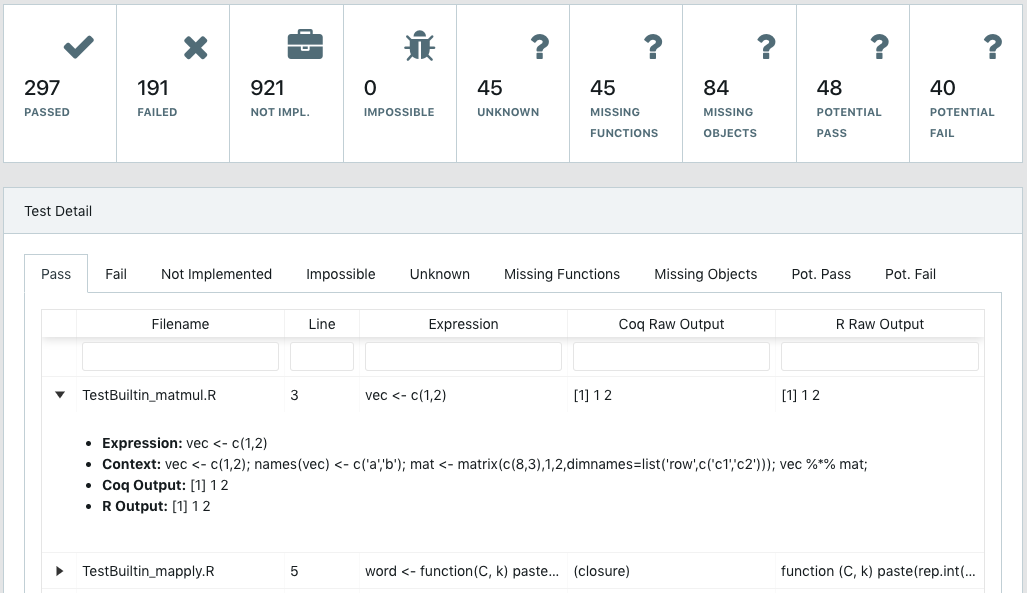
\includegraphics[width=.5\textwidth]{framework.png}
    \caption{Graphical interface of the testing framework}
    \label{fig:testing:interface}
\end{figure}
\noindent\textbf{Testing outcomes.}
After processing, the testing framework obtains the result objects and uses their interface to compare them, returning the corresponding outcome of the comparison.
The testing framework categorizes each step of computation
in one of 7 classes (Figure~\ref{fig:testing:interface}):
%\et{Tomas: please put a screenshot after executing a large test suite}
``passed'', ``failed'', ``not implemented'',
``impossible'', ``unknown'', ``potential pass'' and ``potential fail''.
%
These outcomes denote different possible scenarios in the comparison between GNU~R and \CoqR{}. Beyond the expected ``passed'' and ``failed'',
the ``not implemented'' and ``impossible'' results
correspond to the Coq constructors
\mintinline{Coq}{result_not_implemented} and \mintinline{Coq}{result_impossible}
shown in Figure~\ref{fig:result}. 
As mentioned before, if \CoqR{} were bug free, an ``impossible'' result would correspond to a critical bug in GNU~R---in practice, all the ``impossible'' results we observed were due to mistakes in \CoqR{}.


% \noindent\textbf{Two-step comparison.\td{Not quite, there's the "processing"/"normalization" phase then the comparison}}
% To compare each result, we adopt the general scheme shown in Figure~\ref{fig:methodology}.
% In particular, the comparison of outcomes proceeds in two steps. % First,
% %we identify what {\em type} of result each interpreter returns.
% % I think that this is what Tomás calls ``Processor'', right?
% First, we process the result each interpreter returns and transform\td{maybe normalize is better?}
%  them into a common set of {\em types}.
% Examples of types include errors, boolean vectors, numerical vectors, etc. as well as the special
% ``not implemented'' and ``impossible'' results of \CoqR{}.
% This phase takes care of the necessary normalization in order to obtain meaningful comparison.

% We did not model this logic and therefore sometimes outputs do not match;
% the processor for numerical vectors then converts results by ignoring these subtleties
% (such as spaces).

% These types are then compared; if they do not match,  e.g. if GNU~R returns an error but \CoqR{} returns a string vector, the test is marked as failed without further processing.

% Second, if the two result types are identical
% in both GNU~R and \CoqR{},
% we interpret the results using a type-specific function. Such a function takes care of the necessary normalization in order to obtain meaningful comparison.
% Indeed, \CoqR{}'s pretty-printer is part of the shim (the non-formalized part)
% and does not follow an eyeball correspondence with GNU~R's pretty-printer, which is quite complex. This introduces harmless output mismatches. For instance, when printing vectors with GNU~R, some are left padded, others are right padded. We did not model this logic and therefore sometimes outputs do not match; the normalizer\et{normalizer vs interpreter vs processor} for numerical vectors converts results by ignoring spaces.
% For instance \mintinline{R}{c (1, 100, 2)} is printed
% as \mintinline[showspaces,autogobble=false]{text}{  1 100   2} by GNU~R, while \CoqR{} prints \mintinline[showspaces]{text}{1   100 2  }.
% above
% to the vector \mintinline{R}{c (1, 100, 2)}, ignoring spaces.
% Second, these types are compared; if they do not match,  e.g. if GNU~R returns an error but \CoqR{} returns a string vector, the test is marked as failed without further processing.
% If the two result types are identical in both GNU~R and \CoqR{}, they can be compared for equality.\\
%The final results can be compared for equality after normalization. \\
% leading to either a failure or a success.


% Differences of pretty-printer.
% Let us consider the expression
% \mintinline{R}{x <- c (1, 100, 2); x}.
% There are two steps of execution:
% first the variable \mintinline{R}{x} is assigned a value,
% then it is shown again.
% In the first step,
% the returned value of the assignment operator
% is the assigned value, but is marked as ``invisible'':
% \mb{I chose not to say anything about the parentheses trick:
%     I find invisibility to be a good example of difference in behavior
%     that we had to deal with in the testing framework.}
% it tells the interpreter to temporarily disable its printing.
% We did not model invisibility,
% and our interpreter thus prints \mintinline[showspaces]{text}{1   100 2  }: % I am hiding the [1], yes.
% vectors are just shown by printing its elements,
% all cells being of the same size.
% At the second step,
% our interpreter prints the same value again,
% but GNU~R prints \mintinline[showspaces,autogobble=false]{text}{  1 100   2}:
% some vectors are left padded, other are right padded.
% We did not model this and in this case made the wrong decision.
% %
% However, we still consider that our result is correct,
% and we designed our testing framework to mark it as such.
% % Special cases.
% \noindent{\bf Special categories.}
% It happens that we can not type a result.
% This happens when R produces a result for which we did not
% provide any normalizer.
Sometimes processing a result string fails.
For instance, there exist special attributes that affect
the way vectors are printed, and our pretty-printer is not aware of all of these special attributes. In such cases, the processor fails, and returns an \mintinline{Python}{UnknownResult} object. Such tests are consequently marked as ``unknown''; they could be functionally correct or not, so classifying them apart is practical.
% it would not be correct to mark them as success,
% but it would not be practical to mark them as a failure.
%
% As a special case, \mb{This sentence should be moved before, I think.}
% invisible results (that are thus not printed by R)
% are considered successful whenever \CoqR{} did not return an error.
% Indeed, test suites always include a latter step printing down variables:
% if the computed value is not correct, the testing framework
% will catch it when GNU~R will print down the computed value.

Also, once a single step in a line-by-line test file fails, or leads to a not-implemented result, we cannot say anything about the steps that follow in the test file: subsequent errors and success could both be coincidental.
% Indeed, if we get the same result in both interpreter,
% it could be out of luck:
% they should not be marked as success for correctness.
% otherwise, successful results could suddenly fail
% after correctly implementing a feature.
%
% Symmetrically,
% if such a test fails,
% it could be because the previous step failed---%
% typically if the previous step was an assignment.
% who failed to execute
% and the current step just displays the value of the assigned variable.
Marking such tests as failing would be counter-productive, as
this would lead to a large amount of false positives
in the tests marked as failed.
% (only marked as failing because of a previous failing result).
%
To categorize these tests,
we use the ``potential pass'' and ``potential fail'' outcome categories. These two categories mean nothing for correctness (we cannot conclude anything certain from a potential outcome), but they really help in the development process by showing possible future results.\\


\begin{figure}
    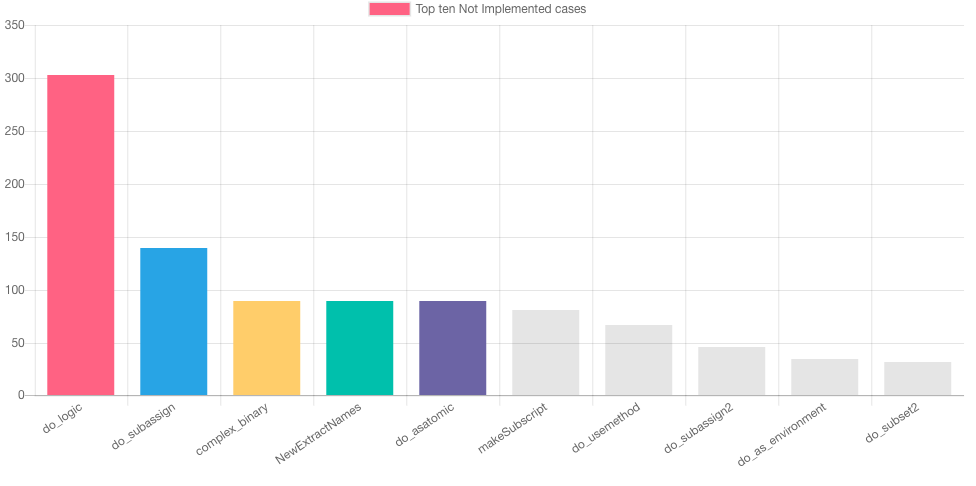
\includegraphics[width=.5\textwidth]{not_implemented_fastr.png}
    \caption{Chart displaying the most needed features to be implemented.}
    \label{fig:library:not_implemented_fastr}
\end{figure}

\noindent\textbf{Guiding the development process.} 
Having different categories of testing outcomes is crucial when facing a huge development, in order to apprehend the task at hand. In particular, we found extremely helpful to separate actual failures from internal uses of \mintinline{Coq}{result_not_implemented}, and from missing function definitions.

Recall that a not-implemented feature generally corresponds to an entry of the symbol table that has not been translated into \CoqR{}. It can also correspond to some branch in a large switch statement that we decided to postpone for some reason. On the other hand, a missing function definition corresponds to the use of an undefined R function in the test; this is typically because the function was not imported in the \CoqR{} test code base. 

Therefore, in addition to counting the classified testing outcomes for the run of a test suite, our testing framework reports two charts reporting respectively the 10 most common not-implemented features (see for instance Figure~\ref{fig:library:not_implemented_fastr}), and, in a similar fashion, the 10 most common missing function definitions. Both reports are useful to identify ``low-hanging fruits'' to make progress in running the selected test suite. For instance, at the initial stages of the project, the base library of R showed up prominently in the list of undefined functions---especially some parts of it, as discussed below.\et{Also useful for scalability: only import needed functions from base library (Coq is slow!)}
Also, we used the report of most used not-implemented features iteratively in order to decide which features from the symbol table to implement first, leading us to the 112 features currently implemented.

%


% How the other results (Potential fail, Not implemented) helped the Coq development.

% \subsection{Driving the Development Process}
% \label{sec:driving:development}


\subsection{Base Library}
\label{sec:library}


% We now report on the effort to allow \CoqR{} to import the base library of R in order to run the test suites of GNU~R and FastR, highlighting how our testing framework helps in this process.

% \noindent\textbf{Description of the base library.}

% The need to execute the base library.

Unsurprisingly, our initial experiments running the test suites of GNU~R and FastR raised a huge number of undefined function errors, whose consolidated report allowed us to locate in the base library of R. As anecdote, having implemented 105 features from the symbol table, more than 80\% of the failures for the GNU~R test suite were still due to missing definitions. After extending \CoqR{} to be able to load the base library, that percentage fell down to about 10\% \et{number}, corresponding to other basic libraries, most importantly the statistics library.

The base library consists of about 160 R source files, totalizing 19,000 lines of code, which are executed by GNU~R prior to any other
expression. This base library includes the definition of several
functions and objects, such as \mintinline{R}{mean}, \mintinline{R}{matrix} or \mintinline{R}{pi}.
Several of these functions are just wrappers over internal functions, adding  argument checking or default arguments. An example is the \mintinline{R}{eval} function which sets default values for the arguments of the internal \mintinline{R}{eval} function:
\begin{minted}{R}
eval <- function(expr, envir = parent.frame(),
    enclos = if(is.list(envir) || is.pairlist(envir))
             parent.frame() else baseenv())
    .Internal(eval(expr, envir, enclos))
\end{minted}

Most of these definitions do not require many features to be implemented in the interpreter in order to be executed: only
the \mintinline{R}{function} keyword and the assignment \mintinline{R}{<-} have
to be implemented.
However, there are other cases where some additional computation
is required on the right-hand side of the assignment.
For instance, the file \texttt{constants.R}
of the base library contains the definition \mintinline{R}{pi <- 4 * atan (1)}.
In order to evaluate this expression, the \mintinline{R}{atan} function has to be implemented.
% We implemented these functions in OCaml.
% (in the case of \mintinline{R}{atan}, by directly using \mintinline{OCaml}{atan}'s functions)
% This is what we call “hooks”.
%These cases are more complex because they usually require features that are not
%implemented by CoqR.
% The base library along with a few others (such as the stats library) prepare the environment needed for GNU~R to run properly.

% \noindent\textbf{Identifying Critical Missing Functions}\et{rename?}
% \label{sec:missing}

Of course, being able to execute the definitions and include
them in the \CoqR{} environment does not mean that these definitions are usable: the internal function called by a library function may not yet be implemented in \CoqR, so if a test executes that function, it will yield a not-implemented result. This is why it is crucial to be able to differentiate real failures from not-implemented results and undefined functions. Note that several functions may end up relying on the same internal (not implemented) feature, giving more meaning to the report of the most common not implemented features.

% %\et{refine/extend/etc.}
% Indeed, the base library is crucial in order to execute the test suites of both GNU~R and FastR. 

% Having implemented 105 features 
% from the symbol table, more than 80\% of the failures for the GNU~R test suite were in fact due to missing definitions. After being able to import the base library,\footnote{Only 3 out of 159 files are currently left out.}, there are no longer failed results due to missing definitions. 

% missing functions from other basic libraries, such as the statistics library.

% the failed results\et{put absolute number: 880?} are  \et{this is without importing anything from the library?} contained in this library. For the FastR test suite, the percentage is around 60\%. In both cases, only 3\% of failures are caused by actual value mismatches (often caused by double precision or string encoding). The remaining percentages correspond to missing definitions due to previous errors in computation.

% In contrast, 
% \et{from the base lib, I guess}. The total number of failed results for the GNU~R tests drops from 880 to 500, corresponding to 

% \et{add the FastR stats (780 what?)}

% \et{relation between missing definitions and not-implemented features?}

% \et{now discuss how things improve -- by implementing more from the symbol table?}


%Once we ran our test suites we noticed that barely 2\% of the failed results
%were due to actual value mismatch (numeric precision, string mismatch), while the
%rest were mostly due to missing functions and objects in our interpreter\td{That percentage is not necessary... But somehow I wanted to say that ~800/870 fails are missing functions}.
% Using one of the features of our framework we identified the most relevant functions
%causing these fails, as can be seen in figure X. We recognized that these belonged
% to the base library loaded by GNU~R interpreter on initialization.


% \subsection{Including the base library to CoqR}
% \label{sec:library:loading}
% The following sections describe the process required to include the base library
% into CoqR's environment.%\td{Meh... Didn't really know how to start this section}
%
% \noindent\textbf{Fix parsing errors.}
% \et{sounds more like an anecdote to me}
% The first step in loading the base library is fixing the parsing errors that arise.
% These errors appear as a consequence of the differences mentioned in section \ref{sec:parsing}.
% One very common error is caused by the syntax used for \mintinline{R}{if else} in the R files,
% considered to be a mistake by GNU~R's own documentation\footnote{By typing \texttt{?Control} in R you get a man page with the warning.}.
% Thus, the files have to be rewritten in order to remove these errors.
% \mbi{We have to be very cautious, here.  Most of the message of this paper is that the R specification is currently not enough
%   because it is not respected in practise by R interpreters.  We thus can't suddenly say that these interpreters are wrong and
%   should be fixed.
%   We can rephrase this by saying that we chose this particular way to keep the parser line-to-line correspondance.}
%
% \noindent\textbf{Implementing missing features.}
% \et{redundant with 4.2 -- integrate what is interesting (features/functions, etc.)}
% As was previously mentioned at the beginning of \ref{sec:library:}, most of the definitions
% can be directly included in CoqR's environment. However, there are some
% functions and objects that need additional computation in order to be defined.
% This additional computation requires features to be implemented in CoqR. These
%  usually correspond to functions found in the symbol table mentioned in
% \ref{sec:coq:structure}.
% %Once this was ready, the definitions had to be included. In particular, there were three files which
% %required many functionalities not yet included to CoqR. Therefore, in order to
% %completely load the base library, the next step was to implement these missing
% %features.
%
% In particular, three files contain most of this additional computation. The definitions
% contained in these files are not of common use in the test suites. Nevertheless,
% to fully load the base library, it is mandatory to implement these required
% features.
%
% % Although we did not count with the whole base library, we ran our test suites to verify
% % our suspicions. We reduced the failing results from around 800 to 500
% % and increased our not-implemented results from 200 up to 700 for the GNU~R test suite.
% % The failing results were mainly due to missing objects caused by computations not performed.
% % For the fastR test suite we obtained ...
%
% \noindent\textbf{Debugging process.}
% \et{is there anything more than anecdotes here?}
%
% Several bugs arise from the process of implementing the missing features. Some of
% these may be easy to fix while others are deeply incrusted in the internal mechanism
% of CoqR. Amongst these last, there are some that produce erroneous results and others
% that could cause CoqR to get stuck.
%
% The Bisect~\parencite{bisect} coverage tool for OCaml proves to be indispensable
% in the fine-grained process of debugging.
% It allows tracking down and identifying evaluation paths which result in execution errors.
% Using custom tests it is possible to reproduce particular expressions not covered by
% the test suites. Finally, using the testing framework allows for a general overview
% of the whole process.
%
%
% One particular case was the implementation of the \mintinline{R}{do_substitute} feature.
% Direct usage of this function would return a valid result. However, using it inside
% of another function would always result in an erroneous value. This is problematic as
% \mintinline{R}{do_substitute} is required by other functions in the base library.
% It was through the combined usage of the aforementioned tools that it
% was possible to identify the main source of error.
% The bug was located at the core of how function calls are made. In particular, it
% was contained in the function responsible for argument matching. As it was finally
% figured, the bug was due to setting some general purpose bits incorrectly at certain
% points in an array.
%





%
%
% Including the three missing files proved to be a richer experience than expected.
% On one hand, implementing the missing features, several deep-incrusted internal bugs
% arose which may have not with the test suites. These bugs would range from
% erroneous results to our interpreter getting stuck. Some would be small and some
% would be at the core of how functions were executed. The bisect
% tool proved to be indispensable in the fine-grained process of debugging, allowing us
% to track down and identify evaluation paths which resulted in execution errors.
% Our set of custom tests would also let us reproduce particular expressions causing
% these erroneous results. Finally our framework would serve particularly in overviewing
% the whole process.

% On the other hand, we noticed a convergence in the functionalities required to load
% the whole base library and the low-hanging fruits detected by our interpreter and
% the test suites.
% We could then cover both aspects at the same time.



\subsection{Current Status}
\label{sec:testing-results}

\et{update, put table with all test suites, and categories of results. Discuss.}



In order to fully include the base library, 9 features from the symbol table had to
be implemented, extending it from 105 to 114 entries.

The results of our tool are available at \url{https://coqr.dcc.uchile.cl}.\mbi{
    OK: we should discuss on what should be the state of this page once the paper
    is published.
    I guess that we should hide some old tests, for instance.
    Should we put a link the source code too? I think it would be nice.}
% We used our testing framework on various test suites\mbi{
%     Outch: it would be nice to explain the test suites here,
%     but at the same time, I like the current flow of the beginning of
%     Section~\ref{sec:test:methodology}.
%     Any ideas?},
We used our testing framework on both the GNU~R test suite and the FastR test suite.
% but also on the base library of R,
% which already provides a large coverage.
%
To evaluate these test suites,
we use the Bisect~\parencite{bisect} coverage tool for OCaml.
Out of the 11,000 program points identified by Bisect,
??\mb{Tomás?} were executed.
We thus think that new test suites are being needed
to complete this coverage.
%
On total,
this testing base contains 4540 steps.
We currently get ??\todo{} success, ??\todo{} not-implemented,
and ??\todo{} unknown.
The failed results in the GNU~R test suite are due to missing functions from other
basic libraries. In particular, most of the functionalities come from the stats
library. For the FastR test suite the failed results are due to double precision.
We get no impossible results in either case.

% We however did get failure and ``impossible'' results
% during our development.
% The causes of these bugs were varied.\mb{It would be nice to make some statistics here.}
% Once a bug was identified by the testing framework,
% we tried to identify what was causing this bugs---%
% and in particular, which function was buggy---%
% using similar tests.
% Once the buggy function was identified,
% we compared its code line by line with the original function from GNU~R.
% In most cases, this was enough to solve the bug.

Due to the various ways GNU~R's pretty printer works, there is a large number of
printing modes and possible results. Our testing framework thus categorizes
many cases as  ``unknown'' (leading to potential passes and failures in the next steps).
However, we designed our framework so it would be simple to add a particular type of result
if a user would need it.

Loading the base library into \CoqR{}'s environment requires around 15 hours.\et{talking about hours is meaningless if you don't give technical description of the execution environment}
Executing the GNU~R and FastR test suites take around 8h each.
On the other hand, when including the Bisect tool the amount of time required to load
the base library increases up to 60h. The test suites increase to X and Y, respectively.\td{have to check times... Apparently I forgot to write them down...}\et{the fact that running bisect takes much longer can be mentioned, briefly, but don't focus on that; that's not our job}
%
% \section{Old}
% \subsection{Results}
% \label{sec:test:results}
%
% \eti{haven't touched this section: waiting for Tomas, and final results}
%
% The results of our tool are available at \url{https://coqr.dcc.uchile.cl}.\mbi{
%     OK: we should discuss on what should be the state of this page once the paper
%     is published.
%     I guess that we should hide some old tests, for instance.
%     Should we put a link the source code too? I think it would be nice.}
% We used our testing framework on various test suites\mbi{
%     Outch: it would be nice to explain the test suites here,
%     but at the same time, I like the current flow of the beginning of
%     Section~\ref{sec:test:methodology}.
%     Any ideas?},
% but also on the base library of R,
% which already provide a large coverage.
% %
% To evaluate these test suites,
% we use the Bisect~\parencite{bisect} coverage tool for OCaml.
% Out of the 11,000 program points identified by Bisect,
% ??\mb{Tomás?} were executed.
% We thus think that new test suites are being needed
% to complete this coverage.
% %
% On total,
% this testing base contains ??\mb{Tomás?} steps.
% We currently get ??\todo{} success, ??\todo{} not-implemented,
% and ??\todo{} unknown.
% But we get\mb{hopefully} no failure or ``impossible'' result.
%
% We however did get failure and ``impossible'' results
% during our development.
% The causes of these bugs were varied.\mb{It would be nice to make some statistics here.}
% Once a bug was identified by the testing framework,
% we tried to identify what was causing this bugs---%
% and in particular, which function was buggy---%
% using similar tests.
% Once the buggy function was identified,
% we compared its code line by line with the original function from GNU~R.
% In most cases, this was enough to solve the bug.
%
% Due to the various ways GNU~R's pretty printer works, there is a large number of
% printing modes and possible results. Our testing framework thus categorizes
% many cases as  ``unknown'' (leading to potential passes and failures in the next steps).
% However, we designed our framework so it would be simple to add a particular type of result
% if a user would need it.
%
% %Our testing framework categorized a large number of cases
% %as ``unknown'' (leading to potential passes and failures in the next steps).
% %This is due to the various ways GNU~R's pretty-printer works.
% %We added several new result processors in our framework
% %to cover more types.
% %We found that extending our framework was easy,
% %but that at the same time there were a large number of printing mode in GNU~R.
% %We thus left these unknown case,
% %knowing that it would be easy to add a particular type of result
% %if a user would need it.
%
%
% \section{Base Library}
% \label{sec:library}
%
% \subsection{Description}
% \label{sec:library:description}
%
% % The need to execute the base library.
% Prior to executing any expression, GNU~R performs a lot of actions.
% First, the heap is initialized.
% This process involves initializing most global variables.
% Then, GNU~R executes the base library.
% It is a group of files written in R,
% totalizing 19,000 lines of code.
% %
% This means that we have to be able to run the base library
% to correctly test our interpreter.
% For instance, without the base library,
% no variable named \mintinline{R}{T} is defined:
% running the program \mintinline{R}{T} results in a lookup error
% in our interpreter whilst resulting in \mintinline{R}{TRUE} in R.
% After running the base library,
% which includes a line of the form \mintinline{R}{T <- TRUE},
% our interpreter behaves as R on this same program.
%
% % Example of typical function definition in the base library.
% Most of these functions are just links to internal functions
% with some argument checking or default arguments.
% Below is an example:
% the base library function \mintinline{R}{eval} behaves very similarly
% to the internal \mintinline{R}{eval} function.
% The difference is that the base library function checks the value of its parameters when determining their default values, before calling the internal function.
% \begin{minted}{R}
% eval <- function(expr, envir = parent.frame(),
%     enclos = if(is.list(envir) || is.pairlist(envir))
%              parent.frame() else baseenv())
%     .Internal(eval(expr, envir, enclos))
% \end{minted}
%
% % About the not-implemented results.
% These definitions are easily run:
% only the \mintinline{R}{function} keyword is necessary
% to define the base library function \mintinline{R}{eval}. Because the internal \mintinline{R}{eval}
% function is already implemented, it is safe to call the base library function.
% In some other cases, the internal functions are not yet implemented in \CoqR, hence calling the base library counterpart results in
% a not-implemented result.
% %However, once the base library has been executed,
% %a not-implemented exception will be thrown
% %if one actually calls the function \mintinline{R}{which}.
% %Indeed,
% %the internal function \mintinline{R}{.Internal (which (x))}
% %has not yet been implemented.
% %
% % This behavior is expected.
% It may seem pointless to execute a function definition
% that our interpreter cannot execute without failing.
% The reason is that failing because of non-implemented features
% is harmless: we know that this result can be safely ignored,
% and our testing framework reports it as such (Section~\ref{sec:testing:architecture}).
% On the other hand, if we had not executed the base library,
% then the interpreter would have failed with an error stating that a function is missing, whilst GNU~R runs successfully.
% Such a difference of behavior would be reported
% as a bug by our testing framework,
% whilst a not-implemented result is not.
% Being able to run the base library thus ensures
% that the testing framework correctly classifies
% the results of \CoqR{}.
%
% % Computational content in the base library.
% The base library also prepares the base environment.
% For instance, the file \texttt{constants.R} of the base library
% contains the \mintinline{R}{pi} definition, shown below.
% Such definitions are more complex as they involve computations:
% to be able to run the base library,
% we need to implement the \mintinline{R}{atan} function---%
% in this case, using an OCaml hook.
% Other features that had to be implemented
% to run the base library
% include functions to create new environments,
% logical operators,
% the \mintinline{R}{substitute} function,
% the \mintinline{R}{$} operator \ignore$% Added to help my TeX syntax highlighting…
% (which fetches an identifier in a named list or an environments),
% as well as various internal functions.
% \begin{minted}{R}
% pi <- 4 * atan (1)
% \end{minted}
%
% % Result.
% We have been able to run the entire base library.
% We believe that this is an evidence that we caught a sizeable
% part of the language features.
%
% \subsection{Development Process}
% \label{sec:library:development}
%
% \mb{Tomás: can you check that what I wrote is indeed right?}
%
% The base library was not added in one block.
% At first,
% almost none of the computational content of the base library passed.
% %
% We found that the design of our testing framework
% could be adapted to help us prioritize the implementation
% of this computational content.
% We found that it was easy to add these features to our framework,
% validating its reusability.
% We believe that this study
% served as a real-world case study for our testing framework.
%
% Indeed,
% it was simple to extract all the steps of the test suites
% that fall into the ``not-implemented'' class,
% then regroup them depending on the not-implemented features.
% %We did it through JSON queries and regular expressions
% %on the stored Coq outputs.
% %
% Figure~\ref{fig:interface:not:implemented} shows a typical example
% of the graphs produced by our framework.
% Few functions here trigger
% most of the not-implemented results:
% the \mintinline{Coq}{do_for} and \mintinline{Coq}{R_POW}
% functions\td{This might have to be updated. do for was partly implemented for the zzz file in base lib}
%  are being used at lot in our test suites,
% without them being implemented.
% This often happened in practise.
% This lead us to quickly identify low-hanging fruits,
% driving the development process forwards.
% %
% Once these functions were implemented,
% this usually led to a large number of results
% switching classes from not-implemented
% to either pass, fail or even new not-implemented cases for other functions
% which could not be executed previously (due to execution stopping earlier).
% We could then focus on the failing new results,
% catching bugs early in development.
% We believe that without this tool,
% we would only have caught bugs in a large development,
% where debugging is much harder.
%
% \begin{figure}
%     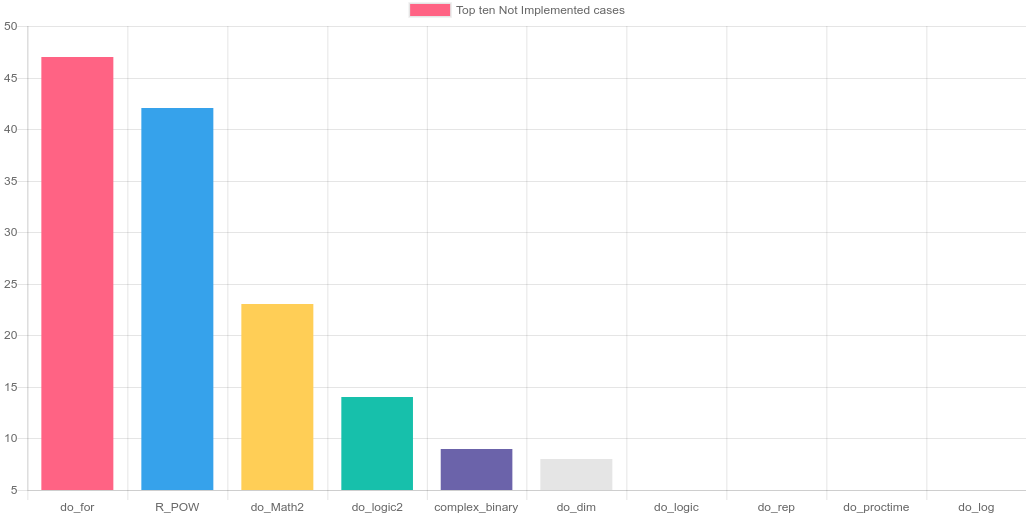
\includegraphics[width=.5\textwidth]{not-implemented.png}
%     \caption{Identifying needed features}
%     \label{fig:interface:not:implemented}
% \end{figure}
%
% We implemented a similar feature for a different issue:
% before all features of the base library were implemented,
% it was difficult to interpret the results of the test suites.
% Indeed, a failing result could be due to either
% a real bug in the \CoqR{} interpreter,
% or be due to it being run without including the base library.
% %
% For instance, most of the fails in which
% the \CoqR{} interpreter resulted in a look-up error
% were due to the missing base library:
% a function should have been defined by running the library.
% %
% We implemented similar graphs than Figure~\ref{fig:interface:not:implemented}
% showing which functions were missing most of the time.
% This led us to identify which part of the base library
% were used in the test suites,
% enabling us to focus on making these part runnable in \CoqR{}.



\section{Formal Reasoning about R}
\label{sec:proofs}

We now address one of the objective stated in the introduction:
our operational semantics should be usable to build proofs about the R language. This section describes one use case:
proving that invariants about the state of the memory are preserved during execution. We also discuss the associated need for proof automation.

As described in Section~\ref{sec:heap},
each basic language element in R is associated one of 24 types,
and each of these types are differently stored in memory.
Figure~\ref{fig:invariants:definition} shows a snippet
of our invariants defined by the \mintinline{Coq}{safe_SExp} inductive property.
%
The constructor \mintinline{Coq}{safe_ListStruct} captures the requirements on well-formed lists. The requirements are expressed using the predicate \mintinline{Coq}{may_have_types S l p}, which
states that the pointer \mintinline{Coq}{p}
is associated in the state \mintinline{Coq}{S} with an object
whose type is in the list \mintinline{Coq}{l}. Hence, the hypothesis on \mintinline{Coq}{cdr} states that the tail of a list is either a list
(\mintinline{Coq}{ListSxp}) or nil (\mintinline{Coq}{NilSxp}).\footnote{The type \mintinline{Coq}{NilSxp} is the type of the \mintinline{Coq}{R_NilValue} global variable (see Section~\ref{sec:globals}); it is used both to end lists and to indicate a missing information.}
Similarly, the constructor states that the tag
of a list is either a character vector or a \mintinline{Coq}{NilSxp} element.
Note that no constraint is specified for the first element \mintinline{Coq}{car} of the list: lists in R are heterogeneous.
%
As another example, the constructor \mintinline{Coq}{safe_StrStruct} states that a string vector contains an array of C pointers,
all of which should be associated with a character vector in memory.

\begin{figure}
\begin{minted}{Coq}
Inductive safe_SExp S : SExp -> Prop :=
  | safe_ListStruct : forall car cdr tag,
    may_have_types S [NilSxp ; ListSxp] cdr ->
    may_have_types S [NilSxp ; CharSxp] tag ->
    safe_SExp S (make_ListStruct car cdr tag)
  | safe_StrStruct : forall data,
    (forall a, Mem a data ->
      may_have_types S [CharSxp] a) ->
    safe_SExp S (make_StrStruct data)
  (* ... *).
\end{minted}
    \caption{Typing invariants for memory} % during R execution
    \label{fig:invariants:definition}
\end{figure}


\begin{figure}
\begin{minted}{Coq}
Lemma do_attr_result :
  forall S globals call op args env,
  safe_state S ->
  safe_globals S globals ->
  safe_pointer S args ->
  may_have_types S [NilSxp; ListSxp] args ->
  (* ... *)
  result_prop (fun S' ans =>
      safe_state S' /\ safe_globals S' globals
      /\ safe_pointer S' ans)
    (do_attr globals runs S call op args env).
Proof.
  introv OKS OKglobals OKargs Targs. unfolds do_attr.
  cutR R_length_result. computeR.
  cutR matchArgs_result. computeR.
  (* ... *)
Qed.
\end{minted}
    \caption{Example of specification and tactic usage.}
    \label{fig:do_attr_result}
\end{figure}

Such invariants are relatively simple, but given the size of the formalization,
they are quite long to establish. Proving that some step of the interpreter preserves the invariants quickly becomes very tedious. In order to address this, we developed various Coq tactics to ease the proof process.
These tactics are mainly useful to propagate known information
through state changes.
 % such operations would have been long and cumbersome for the user, and it automates relatively easily.

Figure~\ref{fig:do_attr_result} illustrates the use of these tactics, with a lemma that states that the \mintinline{Coq}{do_attr} function
defined in Figure~\ref{fig:coq:do_attr} produces a result
that satisfies the invariants.
%
The \mintinline{Coq}{safe_state} predicate specifies
that the given state only stores objects that satisfy the invariants, and similarly
for the global variables of \mintinline{Coq}{globals} with the predicate \mintinline{Coq}{safe_globals}.
The arguments \mintinline{Coq}{call}, \mintinline{Coq}{op},
\mintinline{Coq}{args}, and \mintinline{Coq}{env} of \mintinline{Coq}{do_attr}
are also assumed to satisfy these invariants,
in addition to being of the expected type.
%
In the conclusion of the lemma, the \mintinline{Coq}{result_prop} predicate enables us
to specify what the resulting state of \mintinline{Coq}{do_attr} should satisfy,
whilst ignoring non-interesting cases
such as \mintinline{Coq}{result_not_implemented} or \mintinline{Coq}{result_bottom}.
% Indeed, reaching one of these results means that the result is out of scope for the  interpreter.
% \et{will turn into a forward ref if we move proof section earlier}
% This is the reason why these are not considered harmful
% during the testing process (see Section~\ref{sec:test:methodology}).
% In the normal result, we state that the invariants are still satisfied.

The proof closely follows the source code of \mintinline{Coq}{do_attr}.
After introducing the hypotheses, the function \mintinline{Coq}{do_attr} is unfolded,
leaving its definition ready to be processed by further tactics.
In Figure~\ref{fig:coq:do_attr}, we can see that \mintinline{Coq}{do_attr}
starts by calling \mintinline{Coq}{R_length}.
In the proof we use the \mintinline{Coq}{cutR} tactic with a lemma about \mintinline{Coq}{R_length}. This novel tactic discharges the premises of the lemma and introduces the resulting state:
only the success case is left, the other kinds of results being transparently propagated.
% As for \mintinline{Coq}{do_attr}, the error case yields \mintinline{Coq}{False}
% and is discharged by the tactic.
The call to \mintinline{Coq}{R_length} is thus rewritten
to a simple expression of the form
\mintinline{Coq}{result_success S' n},
where \mintinline{Coq}{n} is the number returned by \mintinline{Coq}{R_length}.
%
We then apply the \mintinline{Coq}{computeR} tactic.
This is the most important tactic provided by our framework:
it moves forwards in the current expression,
propagating everything that can be propagated.
In the example, it unfolds the \mintinline{Coq}{let%success} monadic binder,
as this binder is now associated by a fully-computed result
---thanks to the \mintinline{Coq}{cutR} tactic.
It also updates all properties known to hold for the previous state \mintinline{Coq}{S}
to the new state \mintinline{Coq}{S'} using the results
of the \mintinline{Coq}{R_length_result} lemma.
For instance, the hypothesis \mintinline{Coq}{safe_pointer S args}
is replaced by \mintinline{Coq}{safe_pointer S' args}.
This transition is not particularly difficult to prove
given the right lemmae, but it can be extremely cumbersome to manually perform this transition for each and every available hypotheses.
%
The proof continues by applying the tactic \mintinline{Coq}{cutR} again
with a lemma about \mintinline{Coq}{matchArgs},
then \mintinline{Coq}{computeR} to propagate the hypotheses. And so on.

We have proven that the invariants are safely propagated throughout the execution of several functions\et{which ones?}. The proof for the whole formalization is still work in progress. Given the size of the formalization,
we consider that proving such simple typing invariants
is already too much work to be entirely manually proven:
automation is necessary to ease the proving process
and deal with such sizes.
%
Building tactics like \mintinline{Coq}{cutR}
and \mintinline{Coq}{computeR} is not complex and helps a lot.
However, in the long run, in order for formal reasoning about R to scale, it will be necessary to develop a program logic on top of \CoqR; this is a major undertaking, towards which \CoqR{} is an essential first step.

% We also found that building the \mintinline{Coq}{cutR}
% and \mintinline{Coq}{computeR} in Ltac---%
% the tactic language of Coq---%
% was relatively straightforward.
% As a consequence, we do not expect major difficulties
% to adapt or build similar tactics for other kinds of proofs.


\section{Related Work}
\label{sec:related:work}

% Few tools about R.
R is a notably difficult programming language~\parencite{RInferno},
whose semantics is constantly moving---%
see for instance the recent addition
of R's alternative representation~\parencite{altrepR}.
In our formalization, we chose to ignore these fast moving parts,
but these parts are used by real-world R programs.
Furthermore, the diversity of R users is such that different R programs
will use very different libraries and features,
as the generally accepted guideline~\parencite{RGuidelines}
does not restrain users about them.
This makes it difficult to build tools for R,
and as a consequence, relatively few tools for R exist
in comparison to the size of its community.

% Genthat.
In particular,
there exist few testing frameworks in R.
The testR project~\parencite{maj2013testr, 2014testr},
which later evolved into the Genthat library~\parencite{genthat},
is based on an interesting way of generating unit tests for R functions.
It starts from a program using the functions to be tested.
It then annotates and executes this program,
storing the trace of the calls to the functions to be tested.
Unit tests are then generated from this trace.
The Genthat library is thus useful to generate tests for a library
given some program using it,
which can then be used to ensure that further versions of the library
do not break existing code.

% FastR
GNU~R is not the only R interpreter that exists.
Many existing interpreters are based on the same C core code,
but use different libraries for linear algebra,
usually optimized for a specific usage.
%
The FastR project~\parencite{kalibera2014fast}  takes a different approach
as it also reimplements the core of the R interpreter, using the Truffle self-optimizing framework~\parencite{wuerthingertruffle}.
FastR is faster than the reference interpreter not only in the linear-algebraic part, but also in the language interpretation layer.
%
FastR agrees with us that the GNU~R interpreter is the reference semantics: any behavioral difference between FastR and GNU~R is considered a FastR bug.

% JavaScript semantics and their trust sources.
To the best of our knowledge, we are the first to provide a mechanized specification of R. But the general goal of formalizing full real-world languages---%
as opposed to small subsets---is not new.
%
JavaScript is a particularly relevant example.
Indeed, empirical analyses
have confirmed that the language features
that are usually ignored in the formalized subsets of JavaScript
are actually important for actual web developers~\parencite{RichardsHBV11}.
%
In the case of JavaScript, there are several trust sources.
First, the language is precisely specified by the ECMAScript specification~\parencite{es2019}.
Second, there exist various test suites~\parencite{test262, mozillatests}
as well as several widely used interpreters.
As a consequence, various formal specifications of JavaScript exist,
each related with some of its trust sources.

% Maffeis et al.
The first full formal semantics of JavaScript~\parencite{aplas08}
is a semantics related to the third version of the ECMAScript specification.
It had a major influence on the definitions of further JavaScript formal
specifications~\parencite{usenix, popl14jscert, popl12-Towards, ses} andalso served as the formal basis to prove the soundness of security-related
JavaScript subsets~\parencite{mmt-esorics09, mmt-oakland10,MMT-CSF-TR09}.
This work was however not mechanized. 
%making it difficult to be used as a basis for other formalization work.

% The Essence of JavaScript.
In parallel, several formal semantics
for JavaScript are based on a JavaScript interpreter~\parencite{Guha2010, js-ml,  kjs, Politz:S5}.
These semantics are related to JavaScript test suites,
either by comparing the results with the expected result,
or by comparing results with widely-used JavaScript interpreters.
These formalizations tend to be easier to build
as testing frameworks already exist.
Furthermore, they are usually easier to understand by non-specialists.
However, such formalizations suffer from all the issues of test suites:
for instance, in JavaScript the \mintinline{javascript}{for}-\mintinline{javascript}{in} feature was then loosely tested,
and its behavior varied from interpreters to interpreters.

% JSCert.
The JSCert formalization~\parencite{popl14jscert}
is an interesting step forward as it was designed
to be related with both the ECMAScript specification and the JavaScript test suites.
The formalization is composed of two parts: a mechanized specification and an interpreter. The JSCert specification is syntactically related with the ECMAScript specification through an eyeball correspondence, and the interpreter passes its test suites.
The specification and the interpreter are related to each other by a Coq proof.
This double-relation provides a large amount of trust to JSCert.
In practice, both relations served to find issues in the JSCert specification,
but also some implementation bugs in other interpreters,
as well as mistakes in the ECMAScript specification.
% Furthermore, JSCert is mechanized:
% this facilitates its reuse for other projects.
% However, this project involved 8 people for a year:
% building both a specification and an interpreter,
% as well as a correctness proof between them, involves a lot of resources.
In \CoqR, we take a different approach by defining the big-step operational semantics as an interpreter: the same definition is both executable and syntactically close to its specification (the GNU~R interpreter).

% CompCert.
The Coq proof assistant has already been used
in a variety of mechanized language formalization projects.
The most well-known is the CompCert project~\cite{Leroy-Compcert-CACM},
a verified optimizing compiler for C.
This compiler is proven to be free of compilation bugs,
leading to safer programs in critical software.
This project comes with a formalization of the C programming language,
as well as the formalizations of the intermediate compilation languages.
%
Due to the compilation nature of the CompCert project,
it was acceptable to restrict the behaviors of the C programming language
in their formalization,
restricting it to the behaviors that will actually be compiled by CompCert.
The Formalin project~\parencite{formalin} is another formalization
of the C language, which aims at precisely listing all the possible behaviors of a C program.

\section{Conclusions}
\label{sec:conclusion}

We present the first formal specification of R, written as an interpreter in Coq. We present the monadic encoding that allows \CoqR{} to be in eyeball correspondence with the GNU~R reference interpreter, provide a testing infrastructure useful to incrementally enrich \CoqR, and show that \CoqR{} can be used to formally reason about R. Considering the number of realistic test cases that \CoqR{} currently passes, and its extensible architecture, we believe that \CoqR{} can be grown \CoqR{} to fully cover R and its main libraries. On the formal reasoning side, \CoqR{} should be the basis on top of which to develop an appropriate program logic, in order to more conveniently reason about R programs. As such, it is a necessary first step towards a robust environment for formal verification of R programs. 

\printbibliography{}

\end{document}
